%%%%%%%% ICML 2022 EXAMPLE LATEX SUBMISSION FILE %%%%%%%%%%%%%%%%%

\documentclass[nohyperref]{article}

% Recommended, but optional, packages for figures and better typesetting:
\usepackage{microtype}
\usepackage{graphicx}
\usepackage{subfigure}
\usepackage{booktabs} % for professional tables
\usepackage{adjustbox}

% hyperref makes hyperlinks in the resulting PDF.
% If your build breaks (sometimes temporarily if a hyperlink spans a page)
% please comment out the following usepackage line and replace
% \usepackage{icml2022} with \usepackage[nohyperref]{icml2022} above.
\usepackage{hyperref}


% Attempt to make hyperref and algorithmic work together better:
\newcommand{\theHalgorithm}{\arabic{algorithm}}

% Use the following line for the initial blind version submitted for review:
\usepackage[accepted]{icml2022}

% If accepted, instead use the following line for the camera-ready submission:
% \usepackage[accepted]{icml2022}

% For theorems and such
\usepackage{amsmath}
\usepackage{amssymb}
\usepackage{mathtools}
\usepackage{amsthm}

% if you use cleveref..
\usepackage[capitalize,noabbrev]{cleveref}

%%%%%%%%%%%%%%%%%%%%%%%%%%%%%%%%
% THEOREMS
%%%%%%%%%%%%%%%%%%%%%%%%%%%%%%%%
\theoremstyle{plain}
\newtheorem{theorem}{Theorem}[section]
\newtheorem{proposition}[theorem]{Proposition}
\newtheorem{lemma}[theorem]{Lemma}
\newtheorem{corollary}[theorem]{Corollary}
\theoremstyle{definition}
\newtheorem{definition}[theorem]{Definition}
\newtheorem{assumption}[theorem]{Assumption}
\theoremstyle{remark}
\newtheorem{remark}[theorem]{Remark}

% Todonotes is useful during development; simply uncomment the next line
%    and comment out the line below the next line to turn off comments
%\usepackage[disable,textsize=tiny]{todonotes}
\usepackage[textsize=tiny]{todonotes}


% The \icmltitle you define below is probably too long as a header.
% Therefore, a short form for the running title is supplied here:
\icmltitlerunning{Submission and Formatting Instructions for ICML 2022}

\begin{document}

\twocolumn[
\icmltitle{Opti-ML: An End-to-End Architecture for \\
ML Guided Inlining for Performance}

% It is OKAY to include author information, even for blind
% submissions: the style file will automatically remove it for you
% unless you've provided the [accepted] option to the icml2022
% package.

% List of affiliations: The first argument should be a (short)
% identifier you will use later to specify author affiliations
% Academic affiliations should list Department, University, City, Region, Country
% Industry affiliations should list Company, City, Region, Country

% You can specify symbols, otherwise they are numbered in order.
% Ideally, you should not use this facility. Affiliations will be numbered
% in order of appearance and this is the preferred way.
\icmlsetsymbol{equal}{*}

\begin{icmlauthorlist}
\icmlauthor{Sam Keyser}{MSOE}
%\icmlauthor{Jonny Keane}{MSOE}
%\icmlauthor{Salvin Chowdhury}{MSOE}
%\icmlauthor{Jeremy Kedziora}{MSOE}
\end{icmlauthorlist}

\icmlaffiliation{MSOE}{Electrical Engineering \& Computer Science, Milwaukee School of Engineering, Milwaukee, WI, United States}

\icmlcorrespondingauthor{Sam Keyser}{keysers@msoe.edu}

% You may provide any keywords that you
% find helpful for describing your paper; these are used to populate
% the "keywords" metadata in the PDF but will not be shown in the document
\icmlkeywords{Machine Learning, Reinforcement Learning, Compilers}

\vskip 0.3in
]

% this must go after the closing bracket ] following \twocolumn[ ...

% This command actually creates the footnote in the first column
% listing the affiliations and the copyright notice.
% The command takes one argument, which is text to display at the start of the footnote.
% The \icmlEqualContribution command is standard text for equal contribution.
% Remove it (just {}) if you do not need this facility.

\printAffiliationsAndNotice{}  % leave blank if no need to mention equal contribution
%\printAffiliationsAndNotice{\icmlEqualContribution} % otherwise use the standard text.

\begin{abstract}
FOO BAR BAZ
\end{abstract}

\section{Introduction}
\label{introduction}
LLVM is a modern framework for creating compilers. It decouples the parsing of source code from the generation of valid machine code by introducing an intermediate representation (IR) that captures program semantics in a language agnostic format \cite{llvm-paper}. LLVM is also an optimizing compiler. It performs several passes on program IR in an attempt to improve program size, runtime, or both. A "pass" is a single traversal through either the complete code, or a segment. These optimizations can be performed at several granularities such as Function, Call Graph, Loop, or Module level \cite{llvm-paper}. Passes can generally either gather information or perform a transformation on the module of code. Some passes may also be run several times, either in sequence or after other passes have been performed to take advantage of new changes introduced by prior passes. Passes have been tenatively organized into pipelines such as -O\{1, 2, 3, s, z\} by compiler authors which optimize for either runtime speed or binary size, at the expense of increased compile time. These pipelines can be quite involved; LLVM's -O3 pass involves approximately 160 optimizations passes which involves optimizations performed at multiple different levels of granularity.

% TODO: should I include a vocabulary section?

Function inlining is one of the fundamental optimizations implemented by modern compilers. Function inlining passes are applied at the function level and examine each call site within the function. The decision is then made to either perform inlining or not. Inlining is the replacement of the callsite with the entire function definition. It can be thought of as "copy-pasting" the function definition wherever the function would have been called. Function inlining can improve runtime performance by removing the overhead of jumping to the caller body from the callsite. Additionally, it can improve the performance of downstream optimization passes such as escape analysis by adding more information the current function context \cite{Theodoridis_Grosser_Su_2022}.

Function inlining can have an impact on both the final binary size and the runtime of the final binary. Inlining small functions or functions which are called very infrequently is usually innocuous. The benefit derived from not having to jump to the function definition outweighs the increase in size from duplicating the function definition at each callsite. It becomes more fuzzy when functions are both large and called frequently. Inlining such functions would likely improve the runtime, but would also increase the final binary size. The answer in such a case is not clear. In fact, the inlining problem can be shown as equivalent to a 0-1 knapsack problem, making it NP-complete \cite{Theodoridis_Grosser_Su_2022}. 

% TODO: need to find a way to introduce the idea of "inlining for size" and "inlining for sped"
Function inlining is traditionally solved by heuristics developed by compiler designers. Designing good heuristics is a non-trivial task, but recent work has shown promise in machine-learned policies as an alternative to manually defined policies \cite{mlgo}. To our knowledge, two prior works have approached function inlining using machine learning methods: MLGO \cite{mlgo} and MLGOPerf \cite{mlgoperf}. MLGO chose to focus on creating a heuristic for inlining for size due to several challenges with training an inlining for speed heuristic. MLGOPerf built on the work done by Trofin et al. and proposed a framework for training inlining for speed agents.

%TODO: I feel like I should describe on MLGOPerf so that the reader has context for this contribution section
%TODO: Notice that the MLGO authors specifically called out embedding as something to try! Really good justification for why we tried IR2Vec
Opti-ML builds on top of the work of Ashouri et al. with the following additions\footnote{While not a novel addition, we also produced an open source implementation of MLGOPerf's training architecture: \href{https://github.com/TrainingAfternoon/opti-ml}{https://github.com/TrainingAfternoon/opti-ml}}:
\begin{enumerate}
    % TODO: this should go somewhere else
    %\item An open source implementation of the MLGOPerf training infrastructure\footnote{https://github.com/TrainingAfternoon/opti-ml}\footnote{This repository is still actively being cleaned up as of the time you are receiving this rough draft. The code will be significantly more documented by the end of week 16}
    \item The collection of a dataset based on CppPerfBenchmarks \cite{cpp-perf-benchmarks} for training inlining for speed agents. We collect this dataset because the dataset used by Ashouri et al. is not openly available. We also make available the infrastructure for collecting datasets of this nature.
    \item The replacement of the feature extraction layer within MLGOPerf's IR2Perf model with an embedding layer, IR2Vec \cite{ir2vec}. MLGOPerf relies on extracting a set of manually chosen features from the compiler, which are fed to their model. IR2Vec  introduces the ability to embed the entire representation of a module of code, potentially providing a much richer representation of the IR.
    \item The use of a xgboost random forest as an alternative to deep neural networks for IR2Perf. We found empirically that the xgboost random forest outperformed the neural network, at least when using the IR2Vec embedding layer. We speculate on why this might be later.
\end{enumerate}

The rest of the paper is organized as follows. Section 2 discusses the architectures of MLGO and MLGOPerf in more detail, as well as IR2Vec and the default inlining heuristic for LLVM. Section 3 provides detail on how we collected our dataset and our proposed inlining-for-speed training scheme as well as the hardware \& software used for training our agent. Section 4 presents the results of our function inlining heuristic against the default inlining heurstic and the MLGO v1.0 agent. Finally, section 5 discusses current shortcomings, challenges, and proposes future work. Section 6 concludes the paper.

%Opti-ML builds upon these efforts by creating a full implementation of the MGLOPerf inlining-for-speed training infrastructure, as well as a dataset based on CppPerformanceBenchmarks \cite{cpp-perf-benchmark}. Finally, Opti-ML also replaces the feature extraction layer within MLGOPerf's IR2Perf network with an embedding layer, IR2Vec \cite{ir2vec}.

%Opti-ML proposes the following 
%\begin{enumerate}
%    \item The replacement of the feature extraction layer within MLGOPerf's IR2Perf model with an embedding layer, IR2Vec \cite{ir2vec}. MLGOPerf relies on the 
%\end{enumerate}

%This work builds upon previous efforts to develop a policy for the function inlining optimization pass in the LLVM C/C++ compiler  \cite{mlgo, mlgoperf}.

%These optimizations can be performed at several granularities such as Function, Call Graph, Loop, or Module level \cite{lattner2008}.
%Optimizing compilers use heuristics to guide optimizations such as register allocation and function inlining. These heuristics are frequently hand crafted by experts \cite{TODO} and are sometimes augmented with compile-time feedback from Profile Guided Optimization (PGO)  \cite{PGO}.
%Designing good heuristics is a non-trivial task  \cite{TODO}, but recent work has shown promise in machine-learned policies as an alternative to manually defined policies  \cite{mlgo}. This work builds upon previous efforts to develop a policy for the function inlining optimization pass in the LLVM C/C++ compiler  \cite{mlgo}.

\section{Background}
\label{background}
\subsection{LLVM Inlining Heuristic}
The function inlining pass used by the LLVM C/C++ compiler operates on strongly connected components (SCCs) within the call graph of the module under compilation. Every call in every function is considered for inlining, and a yes/no decision is resolved at each point. Finally, several optimizations are applied on the processed SCC after all inlining decisions have been resolved \as "cleanup" cite{mlgo}. These optimizations can have downstream effects on later inlining decisions.

The inlining decision itself consists of several heuristics. A static cost is estimated for inlining the callee into the caller by simulating post-inlining cleanup passes on the callee. A threshold, estimated based on call site hotness and inlining hints, is applied to the cost to determine the go / no-go decision on inlining the callee \cite{mlgo}. The estimated cost can also be influenced by the number of SIMD instructions within the calee or the number of basic blocks\footnote{A sequence of instructions ending with a yield of control flow. A function can potentially be composed of several basic blocks}. The compiler can also choose to defer an inlining decision, returning the callee back to the queue of call sites to consider, if inlining the caller may result in better savings.

% https://llvm.org/doxygen/Inliner_8h_source.html

% desirability of partial inlining
%A partially inlined function may be desirable in cases where it is called in both very frequently and very infrequently called functions.

\subsection{MLGO}
\subsubsection{Overview}
MLGO, or the "Machine Learning Guided Compiler Optimization Framework" \cite{mlgo}, was an effort to bridge the gap between academic investigation of machine learning methods for compiler optimization and real world compilers. Trofin et al. worked with the LLVM community to introduce a drop-in, machine-learned replacement for the inlining decision heuristic. Trofin et al. chose the inlining decision heuristic for both the importance of the heuristic, and the ease of measuring final binary size compared to a more noisy statistic like program runtime.

Trofin et al. used both reinforcement learning (RL) and evolutionary strategies (ES) to train candidate models for the inlining-for-size heuristic. While Trofin et al. found that the ES method performed slightly better than the RL method, we focus on the RL method in this paper as later work builds on it.

\subsubsection{Reinforcement Learning}
Reinforcement learning is a method for training an agent to understand, and interact with, an environment. The agent, or interchangably the model, learns via trial and error by interacting with its environment. At each time step the agent receives some state $s_t$ which is a collection of features that represent the environment. It takes some action $a_t$ according to its policy, $\pi(s_t)$, which is a distribution over all actions the agent could take conditioned on its current state. After taking an action it receives both its next state and a reward based on the new state, $s_{t+1}, r_{t+1} = \mathcal{R}(s_t, s_{t+1})$. Note that $\mathcal{R}$ is the reward function and is a user designated function. $\mathcal{R}$ is what drives the agent towards a particular goal. In deep reinforcement learning the policy $\pi$ is learned via a deep network which we will represent as $\pi_{\theta}$ where $\theta$ is the parameters defining the model.

Reinforcement learning can also be thought of as solving a Markov Decision Process (MDP), which is a mathematical framework for repesenting sequential decision making problems such as inlining-for-size. The MDP is represented with the 4-tuple $<\mathcal{S}, \mathcal{A}, \mathcal{P}, \mathcal{R}>$. Respectively, $\mathcal{S}$ the set of all states, $\mathcal{A}$ the set of all actions, $\mathcal{P}$ the probability distribution of state transitions $\mathcal{P}(s_{t+1}|s_t,a_t)$, and $\mathcal{R}$ the reward function. The goal of RL algorithms is to find some $\pi^*$ that maximizes the total reward\footnote{$\gamma \in [0, 1]$ is the discount factor. MLGO takes $\gamma = 1$, hence we do not discuss it in depth here} $R = \Sigma^{T}_{t=0}\gamma^t r_t$.

Trofin et al modeled inlining-for-size as
\begin{itemize}
\item\textbf{state}\;$\mathcal{S}$: the current call graph and the current call site being visited
\item\textbf{action}\;$\mathcal{A}$: \{0, 1\} where 1 = inline, and 0 = do not inline
\item\textbf{state transition probability}\;$\mathcal{P}$: $\mathcal{P}$ is captured by the compiler. Inlining is a fully deterministic system in that the same compiler will behave the same way each time when resolving an inlining decision on the exact same state.
\item\textbf{reward}\;$\mathcal{R}$: the native size reduction after inlining is taken (or not taken).
\end{itemize}

Trofin et al. used Proximal Policy Optimization (PPO) \cite{ppo} which is a member of the Policy Gradient \cite{pg_algo} family of RL algorithms. Policy Gradient methods directly learn some $\pi_{\theta}$ which is updated via $\nabla J(\theta)$ where $J(\theta)$ is the expected reward under $\pi_{\theta}$.

% TODO: I should probably come back and explain the full PPO if I have the space
In the interest of simplicity we explain a policy gradient algorithm called REINFORCE \cite{REINFORCE} here. PPO is an enhancement on REINFORCE and the full details can be found in \cite{ppo}.

$\nabla_{\theta}J(\theta)$ is computed as:
\begin{equation} \label{eq:reinforce}
    \nabla_{\theta}J(\theta) = \mathbb{E}\left[\Sigma^{T}_{t=0}R\nabla_{\theta}log\pi_{\theta}(a_t|s_t)\right]
\end{equation}

In practice this expectation is approximated with Monte Carlo methods using $n$ trajectories\footnote{A trajectory, or an episode, is a sequence of $(s_0, a_0, r_1, s_1, a_1, ..., a_{T-1}, s_T, r_T)$ and the total reward $R$}. $\theta$ is updated as:
\begin{equation}\label{eq:updatetheta}
    \theta \leftarrow \theta + \alpha\frac{1}{n}\Sigma^{n}_{i=1}\bigl\{\Sigma^{T}_{t=0}R_{i}\nabla_{\theta}log\pi_{theta}(a_{i,t}|s_{i,t})\bigr\}
\end{equation}
Note $\alpha$ is the learning rate.

Trofin et al. made one change on top of PPO. Because of difficulties in getting native size rewards at each step of the inlining process, they replaced the partial reward with the total reward $R$ in equation \ref{eq:reinforce} \cite{mlgo}.

In addition, due to the complexity of the state space, Trofin et al. simplified $\mathcal{S}$ to a set of 11 numerical features.

Finally, Trofin et al. used imitation learning to "warmstart" the RL agent to imitate the behavior of the default inlining heuristic. This is speed the agent's training by giving it a good baseline policy.

%Additionally, Trofin et al. added infrastructure to the LLVM C/C++ compiler to expose inlining decision data which can be used for training a model. Trofin et al. chose to focus on inlining-for-size, or using the inlining pass to minimize binary size.

%use machine learning to replace the handcrafted heuristics for select compiler optimizations, including function inlining. 

%Trofin et al worked with the LLVM community to develop infrastructure for the clang C/C++ compiler for ingesting ML models as TensorFlow saved models, and the exfiltration of traces for training purposes. Their work was upstreamed into LLVM

%introduce machine learning guided compiler optimizations into a "real world" compiler environment. The authors worked with the LLVM community to develop infrastructure for the clang C/C++ compiler for ingesting ML models as TensorFlow saved models, and the exfiltration of traces for training purposes. Their work was upstreamed into LLVM and used for developing ML-based heuristics for the function inlining and register allocation optimization passes.

%The authors explored two methods for training models in conjunction with the data exposed from the compiler: Proximal Policy Optimization (PPO) \cite{schulman2017proximal}, which is a reinforcement learning (RL) algorithm, and evolutionary strategies (ES) \cite{salimans2017evolution}. We focus on describing Proximal Policy Optimization in this paper, as only the PPO training code was released by Trofin et al.\footnote{\href{https://github.com/google/ml-compiler-opt}{https://github.com/google/ml-compiler-opt}} and later work building on MLGO also use the PPO training strategy.

%Proximal Policy Optimization is
%The authors chose to target the LLVM C/C++ compiler and focused on two compiler optimizations: function inlining and register allocation.

% MLGO repo:
%\footnote{Open sourced at \href{https://github.com/google/ml-compiler-opt}{https://github.com/google/ml-compiler-opt}}
%TODO: do we describe PPO here? -- I think we have to so we can describe how rewards for size work so we have context in MLGOPerf

%to support using saved models in the TensorFlow Saved Model format (later changed to Tflite) during the inlining and register allocation passes. These models act as drop in replacements for the heuristics previously used.

%MLGO worked on function inlining as an incidental problem to their efforts to add the framework for using reinforcement learning (RL) to produce compiler heuristics in lieu of a human. They created a heuristic which used function inlining to specifically optimize for final binary size, rather than binary runtime. MLGOPerf built on top of the framework introduced by Trofin et al. in order to train a function inlining agent to optimize for binary runtime.

\subsection{MLGOPerf}
MLGOPerf \cite{mlgoperf} builds on top of the work of Trofin et al. in order to create an inlining-for-speed agent. One challenge identified in the MLGO paper was the difficulty in training for speed as rewards related to program runtime would be collected, and progam runtime is both very noisy and very expensive to collect \cite{mlgo}. Ashouri et al. proposed the addition of a second model, IR2Perf, to estimate program runtime from the IR level which enables the generation of program runtime rewards during MLGO's training process.

Ashouri et al. collected a corpus of IRs using an autotuner, which uses algorithmic search to assist the compiler's optimization passes, to generate different inlining decisions. Ashouri et al. used the SPEC CPU2006 benchmarking dataset \cite{spec2006} as the basis for their corpus.

Each IR example was compiled with instrumentation\footnote{\href{https://clang.llvm.org/docs/UsersManual.html\#profiling-with-instrumentation}{https://clang.llvm.org/docs/UsersManual.html\#profiling-with-instrumentation}} and ran under the Linux perf tool\footnote{\href{https://perf.wiki.kernel.org/index.php/Main\_Page}{https://perf.wiki.kernel.org/index.php/Main\_Page}} in order to collect runtime data. In particular, perf was used to collect $T_{Func}$ and $T_{Total}$ which were the percentage of time spent in an individual function and the total program runtime respectively. The llvm-profdata tool was used to report $N_{Func}$ which was the number of time each function was called. Using these statistics Ashouri et al. computed the runtime of each function:
\begin{equation} \label{eq:fruntime}
    Func_{runtime} = \frac{T_{Total} * T_{Func}}{N_{Func}}
\end{equation}

Using the results of \ref{eq:fruntime} the total speedup of a function compared to the function compiled with no tuning and default compiler settings was computed as:
\begin{equation}
    Func_{speedup} = \frac{Func_{runtime(Base)}}{Func_{runtime(X)}}
\end{equation}
where $X$ denotes an example from the corpus.

The IR, $Func_{speedup}$ pairs were used to train IR2Perf in a supervised fashion. Prior to training, a collection of 20 features were extracted from the IR to be used as input to the model. Redundant data points were also pruned from the dataset, and the data was normalized and scaled. Finally, PCA was applied to the dataset with $PC=7$ components. The motivation for using PCA was the reduce the sparsity of the data. IR2Perf was trained using Mean Squared Error (MSE) loss function for 5000 epochs.

Other than modifying MLGO to use the IR2Perf network to generate runtime rewards, the MLGO training architecture was left unchanged.

%An issue identified by the MLGO paper with training an inlining-for-speed agent was the development of a good proxy for speed. Benchmarking code modules is very time expensive, which would make training prohibitive except on specially selected datasets \cite{mlgo}. Ashouri et al. proposed the addition of a second model, IR2Perf, which predicts an estimate of binary runtime based on the IR \cite{mlgoperf}.

\subsection{IR2Vec}
IR2Vec is a general purpose embedding model for LLVM IR \cite{ir2vec}. Embedding models are models which try to learn a transformation over some distribution that preserves the information within the original domain. They are frequently used in the context of NLP to convert natural language into a numeric format within There are two broad classes of embedding models: context window based, like word2vec \cite{word2vec}, and knowledge graph based, like TransE \cite{transE}. 

Context windows try to infer token meaning using proximal tokens. Knowledge graphs, which use an entity-relationship model, can capture longer range relationships by observing the relationships participated in by each entity. A knowledge graph is composed of triplets $\langle h, r, t \rangle$ where $h, t \in Entities$ and $r \in Relations$. The representations of $h, t$ are learned as translations from the head entity $h$ to the tail entity $t$ via the relation $r$ in a high dimensional embedding space \cite{ir2vec}. Given any pair of the triplet, the third member of the triplet should be recoverable in a properly learned knowledge graph.

% TODO: I really should go and describe the structure of the LLVM IR file in the background section somewhere

IR2Vec uses a knowledge graph based embedding model. Each instruction within the IR file is represented as an entity. Each instruction is considered to participate in the following relations: (1) opcode \& type of the instruction, (2) the opcode \& type of the subsequent instruction, and (3) the relation between the opcode and each of the instructions arguments. More formally, each instruction $l$ can be represented $\langle O, T, A \rangle$ where $O$ is the opcode, $T$ is the type, and $A$ are the arguments of the function $A_1, A_2, ..., A_n$. IR2Vec computes the instruction vector as:
\begin{equation}\label{eq:ir2vec-inst-vec}
    W_o.O + W_t.T + W_a.(A_1 + A_2 + ... + A_n)
\end{equation}
where $.$ is the scalar multiplication operator and $W_o, W_t, W_a$ are scalars $\in [0, 1]$. $W_o, W_t, W_a$ are chosen in accordance with a heuristic such that $W_o > W_t > W_a$.

IR2Vec refers to instruction vectors such as these as "symbolic vectors". The instructions are used in conjunction with TransE to learn a "seed embedding vocabulary" which is used to lookup instruction vectors based on instruction at inference time. There are a second class of instruction vectors which IR2Vec refers to as "flow aware" which make use of the other information within the IR such as $use-def$ (UD) information. UD information encodes the different lifetimes of a variable, or its uses. Variables hich are currently in use are said to be "live". Flow aware embeddings are described in more detail in the original paper \cite{ir2vec}.

Live instruction vectors are grouped by the basic block that they belong to and summed to create basic block level embedding vector. Functions are composed of potentially several basic blocks and can be created in the same way. Similarly, function level embedding vectors can be summed to create a representative vector of the entire module.

%IR2Vec uses a entity-relation model of the IR where individual instructions are entities, and the relations between instructions are edges.

%This can be formalized as a set of triplets $\langle h, r, t \rangle$ where $h$ and $t$ are nodes within the model, and $r$ 

\section{Methods}
\label{methods}
\subsection{Computing Environment}
All work for Opti-ML was performed in a Debian 12 Bookworm VM with a 16-core ARM Neoverse-N1 and 256GiB RAM. A complete list of software packages necessary for setting up the compute environment can be found in the project repository\footnote{\href{https://github.com/TrainingAfternoon/opti-ml}{https://github.com/TrainingAfternoon/opti-ml}}.

\subsection{Data Sources}
\subsubsection{CppPerformanceBenchmarks}
CppPerformanceBenchmarks is a collection of C++ files intended to evaluate C++ compiler performance \cite{cpp-perf-benchmarks}. CppPerformanceBenchmarks consists of 69 distinct benchmarks. We chose a subset of examples which ran in under two minutes: (1) machine.cpp, (2) functionobjects.cpp, (3) loop\_removal.cpp, (4) rotate\_bits.cpp, and (5) scalar\_replacement\_structs.cpp.

We used CppPerformanceBenchmarks as the basis for our training and validation datasets. We chose CppPerformanceBenchmarks because of its (1) free availability, (2) being compatible with the Clang compiler, and (3) it's ease of use.

\subsubsection{cBench}
The Collective Benchmark (cBench) is a collection of open-source programs with an emphasis on portability and support for several compilers such as GCC, LLVM, etc. The cBench collection has been used for evaluating compiler optimizations within MILEPOST GCC before \cite{cbench}.

We used cBench as our testing corpus. It has similar positives to CppPerformanceBenchmarks, as well as being the testing corpus used by MLGOPerf \cite{mlgoperf}.

\subsection{IR2Perf}
\subsubsection{Data Collection}
Unlike MLGOPerf we chose to forgo the use of an autotuner for a few reasons: 1) there were no good open source tuners available for our case, 2) we thought that by instead generating samples under varying inlining conditions we might more uniformly explore the space of inlining configurations, hopefully helping the IR2Perf performance. We hope that providing the infrastructure for collecting corpuses of IR files with different inlining configurations will help efforts in this area.

We varied the default inlining heuristic by modifying the `-inline-threshold` flag. We used thresholds $\tau$ uniformly randomly sampled from $\bigr\{x\;|\;0 \leq x \leq 1000,\;0 \equiv x (mod\;25)\bigr\}$. The inlining threshold controls the cost which a function must stay under to be considered for inlining. Additionally, in order to collect the data for training IR2Perf we compiled each program with `-fno-omit-frame-pointer`\footnote{\href{https://www.brendangregg.com/blog/2024-03-17/the-return-of-the-frame-pointers.html}{https://www.brendangregg.com/blog/2024-03-17/the-return-of-the-frame-pointers.html}} and `-fprofile-generate`.

We then ran each binary to record runtime information. We limited each run to 1 CPU core via numactl. The system page cache was cleared after each run to avoid influencing subsequent runs. During execution the binaries were monitored by the Linux perf tool and run with LLVM profiling enabled.

Linux perf is a event-oriented observability developed for use by Linux kernel developers. It is capable of observing hardware events like CPU performance counters, as well as taking snapshots of current CPU usage using custom timed interrupt events \cite{perf}. We sample with a frequency of 500Hz. We record the number of CPU cycles observed during progam execution, as well as snapshots of the call stack at each sample. This is used to compute an "overhead" value for each function, or how much time is spent within each function during the lifetime of the program.

LLVM profiling injects hooks into the compiled code which report function usage counters. Profiling does have an impact on code runtime as additional instructions are added to the final binary to be executed.

Traces for each function for benchmark file were collected, except when profiling information was not able to be collected. Because of its nature as a sampling profiler, perf was capable of "missing" a function, especially in the faster benchmark files.

Using this method we collected 111,844 total records which we used to train our own IR2Perf network.

\subsubsection{Training}
We trained an XGBoost Random Forest model in lieu of a deep neural network. We empirically found that the Random Forest model fit the data better than a deep regression network, which ended up having numerical issues. Random Forest is an ensemble model which utilizes multiple decision trees which vote together on the final prediction\footnote{\href{https://builtin.com/data-science/random-forest-algorithm}{https://builtin.com/data-science/random-forest-algorithm}}. XGBoost is a method for using gradient boosting to train random forests\footnote{\href{https://xgboost.readthedocs.io/en/stable/tutorials/rf.html}{https://xgboost.readthedocs.io/en/stable/tutorials/rf.html}}.

Our training pipeline was as follows: (1) embed IR file using IR2Vec, (2) drop redundant data points, (3) normalize and scale the embedding vectors, (4) perform PCA with PC=7 on the embedding vectors, and (5) fit the model with MSE loss using the precomputed $Func_{speedup}$ as a target variable.

\subsection{Reinforcement Learning Agent}

We used the same training scheme proposed by Ashouri et al., which modified the PPO algorithm used by MLGO to use the IR2Perf network to generate rewards during execution \cite{mlgoperf}. The MLGO training pipeline was otherwise left unmodified.

We trained the RL agent for 3000 iterations. Each iteration the model collects several pre-inlining IR samples from the corpus. The current policy is used to make inlining decisions on the IR and then a reward is generated using IR2Perf after embedding the IR immediately before it would be lowered to machine code using IR2Vec. The policy is trained on this subset for $num_policy=3000$ iterations using the current policy $\pi_{\theta}$ \footnote{A detailed set of hyperparameters can be seen at \href{https://github.com/TrainingAfternoon/opti-ml/blob/main/compiler\_opt/rl/inlining/gin\_configs/ppo\_nn\_agent.gin}{https://github.com/TrainingAfternoon/opti-ml/blob/main/compiler\_opt/rl/inlining/gin\_configs/ppo\_nn\_agent.gin}} according to algorithm \ref{alg:mlgo}.

\begin{algorithm}
    \caption{Training Inliner RL Model using IR2Perf}
    \label{alg:mlgo}
\begin{algorithmic}
    \STATE \textbf{procedure} FunctionSpeedup
       \FOR{Function f in module}
       \STATE $FTs \leftarrow getFunctionFeatures()$
       \STATE $funcReward \leftarrow infer(FTs)$
       \STATE $totalReward \leftarrow append(funcReward)$
       \ENDFOR
       \RETURN $totalReward$
    \STATE \textbf{end procedure}
\end{algorithmic}
\;
\;
\begin{algorithmic}
    \STATE \textbf{procedure} CallsiteInline
        \STATE initialize policy $\pi_{\gamma}$ randomly
        \FOR{iteration i in Training}
        \STATE $s_i \leftarrow Sample_{\mathcal{N}_{(0,1)}}(TrainingData)$
        \STATE Compile and Get IR with policy $\pi_{\gamma + \sigma_i}$
        \STATE $R \leftarrow FunctionSpeedup(Module)$
        \STATE Update policy $\theta$ using equation \ref{eq:updatetheta}
        \ENDFOR
    \STATE \textbf{end procedure}
\end{algorithmic}
\end{algorithm}

\section{Results}
\label{results}
\subsection{IR2Perf}
The model failed to adequately fit the dataset when trained on the entire collected cpp-perf-benchmarks corpus, as can be seen in figure \ref{fig:ir2perf-fit}. The random forest appears to predict around the mean of the distribution\footnote{In fact it does: $\bar{y} = 0.8755$, $\bar{\hat{y}} = 0.8772$}. We take this as an indication that the network has failed to generalize and is predicting the mean as a means to reduce its MSE loss.

\begin{figure}[h!]
    \centerline{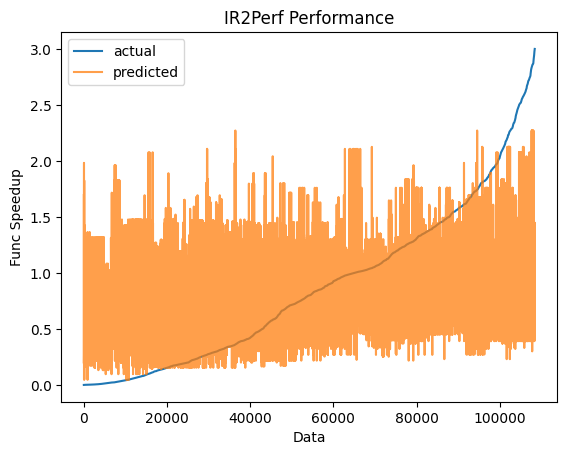
\includegraphics[width=\columnwidth]{ir2perf-fit}}
    \caption{The fit of the random forest model to entire cpp-perf-benchmarks corpus. $R^2 = 0.1367$}
    \label{fig:ir2perf-fit}
\end{figure}

\subsection{Evaluating RL Agent}
We evaluated the default inlining heuristic, v1.0 of the MLGO inlining-for-size policy\footnote{\href{https://github.com/google/ml-compiler-opt/releases/tag/inlining-Oz-v1.0}{https://github.com/google/ml-compiler-opt/releases/tag/inlining-Oz-v1.0}}, and the inlining-for-speed policy we trained. The results of each policy on the training set are included in table \ref{table:cpp-perf-benchmarks} and the results of each policy on the testing set are included in table \ref{table:cBench}.

\begin{table}[h]
    \caption{cpp-perf-benchmarks results}
    \label{table:cpp-perf-benchmarks}
    \begin{tabular}{llrr}
\toprule
                           &        &  mean runtime (s) &  variance \\
file & agent &               &           \\
\midrule
locales & base &      103.6343 &    0.3870 \\
                           & mlgo &      104.1613 &    0.1510 \\
                           & policy &      104.3913 &    0.7208 \\
loop removal & base &      240.0767 &    0.0016 \\
                           & mlgo &      240.0443 &    0.0001 \\
                           & policy &      240.0720 &    0.0002 \\
rotate bits & base &      240.0780 &    0.0004 \\
                           & mlgo &      240.0523 &    0.0001 \\
                           & policy &      240.0767 &    0.0007 \\
scalar replacement structs & base &      240.0680 &    0.0001 \\
                           & mlgo &      240.0547 &    0.0002 \\
                           & policy &      240.0723 &    0.0001 \\
\bottomrule
\end{tabular}
\end{table}

\begin{table*}
%\begin{center}
\caption{cBench results}
\label{table:cBench}

\begin{tabular}[t]{llrr}
\toprule
                &        &  mean\_runtime &  variance \\
file & agent &               &           \\
\midrule
automotive\_bitcount & base &        2.8820 &    0.0000 \\
                & mlgo &        1.4797 &    0.0000 \\
                & policy &        1.4790 &    0.0000 \\
automotive\_qsort1 & base &        4.3207 &    0.0445 \\
                & mlgo &        3.9603 &    0.0680 \\
                & policy &        3.8520 &    0.0010 \\
automotive\_susan\_c & base &        4.3420 &    0.0084 \\
                & mlgo &        4.1477 &    0.3710 \\
                & policy &        3.9800 &    0.0024 \\
automotive\_susan\_e & base &        4.9197 &    0.0120 \\
                & mlgo &        3.6880 &    0.3526 \\
                & policy &        3.6387 &    0.1231 \\
automotive\_susan\_s & base &        3.0677 &    0.0275 \\
                & mlgo &        3.3737 &    0.0300 \\
                & policy &        3.3093 &    0.0229 \\
bzip2d & base &        8.4847 &    1.4539 \\
                & mlgo &       21.0097 &   35.1160 \\
                & policy &        8.0027 &   55.8760 \\
bzip2e & base &        4.8517 &    1.2697 \\
                & mlgo &        4.5333 &    0.0717 \\
                & policy &        3.9097 &    0.0125 \\
consumer\_jpeg\_c & base &        5.6273 &    0.1472 \\
                & mlgo &        5.6213 &    0.0597 \\
                & policy &        5.2290 &    0.1383 \\
consumer\_jpeg\_d & base &       12.1763 &    0.3222 \\
                & mlgo &       10.6993 &    2.3097 \\
                & policy &       11.1373 &    0.4752 \\
consumer\_lame & base &        4.2117 &    0.3088 \\
                & mlgo &        4.0360 &    0.1572 \\
                & policy &        3.7660 &    0.4595 \\
consumer\_tiff2bw & base &        7.5163 &    0.4197 \\
                & mlgo &        7.5157 &    0.3752 \\
                & policy &        8.0403 &    0.3328 \\
consumer\_tiff2rgba & base &       12.7763 &    0.6915 \\
                & mlgo &       12.3693 &    0.3843 \\
                & policy &       12.8823 &    0.3112 \\
\end{tabular}
\;
\;
\begin{tabular}[t]{llrr}
\toprule
                &        &  mean\_runtime &  variance \\
file & agent &               &           \\
\midrule
consumer\_tiffdither & base &        7.5450 &    0.5708 \\
                & mlgo &        7.5607 &    0.1149 \\
                & policy &        7.3280 &    0.3008 \\
consumer\_tiffmedian & base &        4.6420 &    0.0268 \\
                & mlgo &        4.8743 &    0.3393 \\
                & policy &        4.4903 &    0.0948 \\
network\_dijkstra & base &        0.4893 &    0.0010 \\
                & mlgo &        0.5253 &    0.0006 \\
                & policy &        0.4857 &    0.0008 \\
network\_patricia & base &        3.0603 &    0.2653 \\
                & mlgo &        2.4910 &    0.0077 \\
                & policy &        2.3667 &    0.0007 \\
office\_stringsearch1 & base &        3.0513 &    0.0000 \\
                & mlgo &        3.0067 &    0.0000 \\
                & policy &        3.0003 &    0.0000 \\
security\_blowfish\_d & base &        7.7327 &    0.0012 \\
                & mlgo &        7.4707 &    0.0010 \\
                & policy &        7.4700 &    0.0010 \\
security\_blowfish\_e & base &        7.7310 &    0.0000 \\
                & mlgo &        7.5793 &    0.0006 \\
                & policy &        7.5460 &    0.0008 \\
security\_rijndael\_d & base &       34.3053 &    1.2041 \\
                & mlgo &       32.6087 &    1.9962 \\
                & policy &       33.0133 &    1.4967 \\
security\_rijndael\_e & base &       35.8230 &    1.2207 \\
                & mlgo &       34.4080 &    1.0288 \\
                & policy &       30.3487 &    1.3440 \\
security\_sha & base &        6.3510 &    0.0038 \\
                & mlgo &        5.6123 &    0.0059 \\
                & policy &        5.5323 &    0.0026 \\
telecom\_CRC32 & base &        2.4580 &    0.0000 \\
                & mlgo &        2.4640 &    0.0000 \\
                & policy &        2.4530 &    0.0004 \\
telecom\_adpcm\_c & base &        3.9810 &    0.0007 \\
                & mlgo &        4.0097 &    0.0003 \\
                & policy &        4.0137 &    0.0000 \\
telecom\_adpcm\_d & base &        3.8277 &    0.0010 \\
                & mlgo &        3.6897 &    0.0009 \\
                & policy &        3.6970 &    0.0007 \\
\bottomrule
\end{tabular}
%\end{center}
\end{table*}


%TODO: quickly describe what the numbers mean

\section{Discussion}
\label{discussion}
\subsection{IR2Perf}
% TODO: if results are good, talk about ranking
% TODO: if results are bad, talk about IR2Vec being a problem and show figs

\subsection{Future Work}
We have several directions we would like to take this work next. While we observed worse-than-before results from adding IR2Vec to the IR2Perf model, the use of embedding models to represent IR when trying to predict program runtime still seems promising. We could investigate the creation of a custom embedding model for IR2Perf.

Another improvement could be the introduction of partial rewards to the PPO algorithm described in equation \ref{eq:REINFORCE}. MLGO opted to approximate partial rewards with the total reward $R$ because of the challenges with generating a partial reward for each inlining decision, but this is a deviation from the proper algorithm. Using IR2Perf we should be able to generate partial rewards by running the IR through the model after each inlining decision instead of after all decisions have been made.

Finally, %TODO: finish this thought


\section{Conclusion}
\label{conclusion}
\begin{itemize}
\item Summarize takeaways\@.
\end{itemize}

% Acknowledgements should only appear in the accepted version.
\section*{Acknowledgements}

Thank you to the members of the Kedziora Research Lab for feedback and suggestions through out the process: Jonny Keane, Dr. Jeremy Kedziora, and Salvin Chowdhury.

Thank you to the members of the capstone committee for supervising this work: Dr. John Bukwoy, Dr. Rob Hasker, and Dr. Jeremy Kedziora.

Finally, thank you to Dr. RJ Nowling for providing the computing platform used during this work.

% In the unusual situation where you want a paper to appear in the
% references without citing it in the main text, use \nocite
\nocite{langley00}

\bibliography{final-report}
\bibliographystyle{icml2022}


%%%%%%%%%%%%%%%%%%%%%%%%%%%%%%%%%%%%%%%%%%%%%%%%%%%%%%%%%%%%%%%%%%%%%%%%%%%%%%%
%%%%%%%%%%%%%%%%%%%%%%%%%%%%%%%%%%%%%%%%%%%%%%%%%%%%%%%%%%%%%%%%%%%%%%%%%%%%%%%
% APPENDIX
%%%%%%%%%%%%%%%%%%%%%%%%%%%%%%%%%%%%%%%%%%%%%%%%%%%%%%%%%%%%%%%%%%%%%%%%%%%%%%%
%%%%%%%%%%%%%%%%%%%%%%%%%%%%%%%%%%%%%%%%%%%%%%%%%%%%%%%%%%%%%%%%%%%%%%%%%%%%%%%
%\newpage
%\appendix
%\onecolumn
%\section{Policy Results on Training / Testing Corpii}

%%%%%%%%%%%%%%%%%%%%%%%%%%%%%%%%%%%%%%%%%%%%%%%%%%%%%%%%%%%%%%%%%%%%%%%%%%%%%%%
%%%%%%%%%%%%%%%%%%%%%%%%%%%%%%%%%%%%%%%%%%%%%%%%%%%%%%%%%%%%%%%%%%%%%%%%%%%%%%%


\end{document}


% This document was modified from the file originally made available by
% Pat Langley and Andrea Danyluk for ICML-2K. This version was created
% by Iain Murray in 2018, and modified by Alexandre Bouchard in
% 2019 and 2021 and by Csaba Szepesvari, Gang Niu and Sivan Sabato in 2022. 
% Previous contributors include Dan Roy, Lise Getoor and Tobias
% Scheffer, which was slightly modified from the 2010 version by
% Thorsten Joachims & Johannes Fuernkranz, slightly modified from the
% 2009 version by Kiri Wagstaff and Sam Roweis's 2008 version, which is
% slightly modified from Prasad Tadepalli's 2007 version which is a
% lightly changed version of the previous year's version by Andrew
% Moore, which was in turn edited from those of Kristian Kersting and
% Codrina Lauth. Alex Smola contributed to the algorithmic style files.
